\section{zk-SNARK}

L'acronimo zk-SNARK rappresenta l'espressione completa "Zero Knowledge Succinct Non-Interactive Argument of Knowledge".
Questa tecnologia è stata formalizzata per la prima volta in un articolo scientifico pubblicato nel 2014 intitolato
"Succinct non-interactive Zero Knowledge for a von Neumann architecture"\cite{10.5555/2671225.2671275}. Da allora, sono state apportate diverse migliorie alla tecnologia
e sono emerse numerose applicazioni in svariati settori. Le prime applicazioni significative di zk-SNARK sono state
implementate nel contesto della Blockchain, che rimane il settore dove la tecnologia è più conosciuta e applicata. Per
fare alcuni esempi Ethereum\footnote{\url{https://ethereum.org}} una delle Blockchain più accreditate,  ha iniziato ad implementare la tecnologia nella sua
rete dal 2016, e il suo fondatore Vitalik Buterin ha scritto in un articolo sull’argomento: “Perhaps the most powerful
cryptographic technology to come out of the last decade is general-purpose succinct Zero Knowledge proofs, usually
called zk-SNARKs” \cite{how-zk-snarks-are-possible} (Forse la tecnologia crittografica più potente emersa nell'ultimo decennio è quella delle prove
concise a conoscenza zero di uso generale, solitamente chiamate zk-SNARK.).

Zk-SNARK, come suggerisce il nome, rappresenta una tecnologia fondata sul protocollo crittografico Zero Knowledge proof,
il quale consente a una parte (il dimostratore) di dimostrare a un'altra (il verificatore) la veridicità di
un'affermazione senza rivelare nessuna informazione ulteriore. Inoltre questo processo di dimostrazione, viene
effettuato in modo da ottenere una prova, in cui : sia la dimensione della prova, che il tempo necessario per verificarla
crescono molto più lentamente rispetto al calcolo da verificare e senza la necessità di interazione bidirezionale tra le
due parti coinvolte.

Di seguito esamineremo meglio le singole parti che compongono la tecnologia zk-SNARK, analizzando i suoi componenti
chiave per ottenerne una panoramica completa.

\textbf{Notare}: Nei prossimi paragrafi lavoreremo nel dominio algebrico dei campi finiti.

\subsection{Zero Knowledge}

Come accennato precedentemente, Zero Knowledge proof è un protocollo crittografico in cui una parte dimostra di
conoscere una determinata informazione a un'altra parte, senza rivelare alcuna informazione aggiuntiva su di essa. Per
esempio, se Peggy vuole dimostrare a Victor di conoscere la password del suo account, senza rivelargli la password stessa,
può utilizzare un protocollo di tipo Zero Knowledge. In questo modo, Peggy può dimostrare a Victor di sapere quale è la
password corretta senza rivelarla, proteggendo così la sua privacy e la sicurezza del suo account.

Formalmente le prove di tipo Zero Knowledge non sono dimostrazioni di carattere matematico, ma probabilistiche, il che
significa che c'è sempre una probabilità che un dimostratore disonesto riesca a dimostrare la veridicità di
un'affermazione a un verificatore onesto. Esistono tuttavia tecniche per ridurre questa probabilità a valori piccoli a
piacere.

Il primo articolo che definisce il costrutto è “The Knowledge Complexity of Interactive Proof-Systems"\cite{10.1145/22145.22178} pubblicato nel
1985, dove  gli autori introducono il concetto di “Zero Knowledge proof” come un tipo di "interactive proof
systems" \cite{interactive_proof_system} (un modello computazionale che simula lo scambio di
messaggi tra due individui) in cui il verificatore non apprende nulla oltre alla verità dell'affermazione che viene
dimostrata.

Per poter ottenere un sistema Zero Knowledge proof per una particolare affermazione abbiamo bisogno che la prova
generata soddisfi le seguenti proprietà :
\begin{itemize}
    \item \textbf{Completezza}: Se l'affermazione da dimostrare è vera, allora un verificatore onesto (cioè che segue correttamente le
    regole del protocollo) verrà convinto della veridicità da un dimostratore onesto.
    \item \textbf{Correttezza}: Se l'affermazione è falsa, nessun dimostatore disonesto può convincere un verificatore onesto che essa è vera, se non con una piccola
    probabilità.
    \item \textbf{Zero Knowledge}: se l'affermazione è vera, nessun verificatore apprende altro se non il fatto che
    l'affermazione è vera.
\end{itemize}
Le tre proprietà appena viste descrivono un sistema Zero Knowledge proof da un punto di vista formale ma per avere una visione più
intuitiva del protocollo è utile vederne il funzionamento attraverso un esempio. L’esempio in questione è tratto
da un famoso articolo di Jean-Jacques Quisquater "How to Explain Zero Knowledge Protocols to Your Children” \cite{10.1007/0-387-34805-0_60}  ne
estrapolerò solo le parti essenziali alla trattazione, ma ne consiglio la lettura.

L’esempio riguarda una caverna a forma di anello, nella quale è posta a metà del percorso una porta che impedisce il
passaggio, a meno di non conoscere una parola segreta. Supponiamo l'esistenza di due parti, Peggy - che
conosce il segreto della porta e agirà da dimostratrice - e Victor - che invece non conosce il segreto e sarà il
verificatore. Peggy vuole dimostrare a Victor di sapere come superare la barriera senza però rivelare il segreto. Per
fare ciò, Peggy propone a Victor di seguire una strategia: dapprima stabiliscono un nome per identificare i due percorsi
(ad esempio, A e B), poi Victor rimane fuori dalla caverna mentre Peggy sceglie uno dei due percorsi. 
\begin{figure}[H]
    \centering
    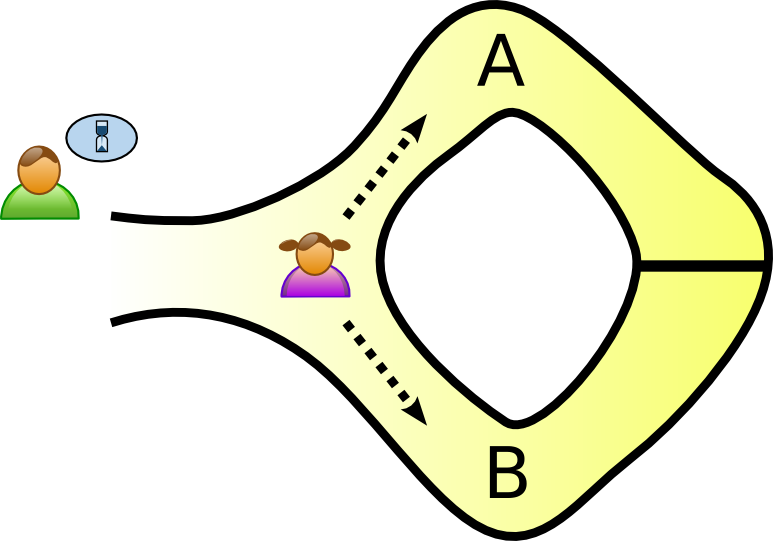
\includegraphics[width=5cm]{./chapters/1.state-of-art/images/5.1.alibaba_cave.png}
    \label{fig:alibaba-cave1}
    \captionsetup{justification=centering}
    \caption{ZKP: Alibaba Cave}
\end{figure}
Dopo qualche minuto, Victor entra nella caverna e chiama ad alta voce il nome di uno dei due percorsi, a quel punto Peggy dovrà
uscire dal percorso chiamato da Victor. 
\begin{figure}
    \centering
    \begin{subfigure}{.5\textwidth}
        \centering
        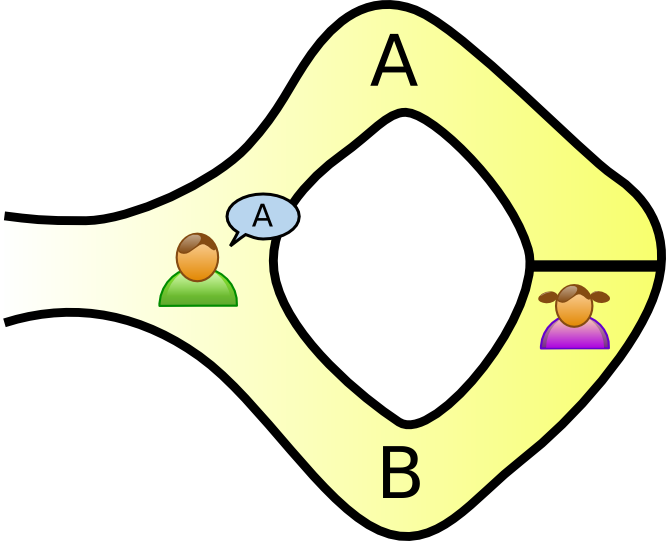
\includegraphics[width=4cm]{./chapters/1.state-of-art/images/5.2.alibaba_cave.png}
        \label{fig:alibaba-cave2}
        \captionsetup{justification=centering}
    \end{subfigure}%
    \begin{subfigure}{.5\textwidth}
        \centering
        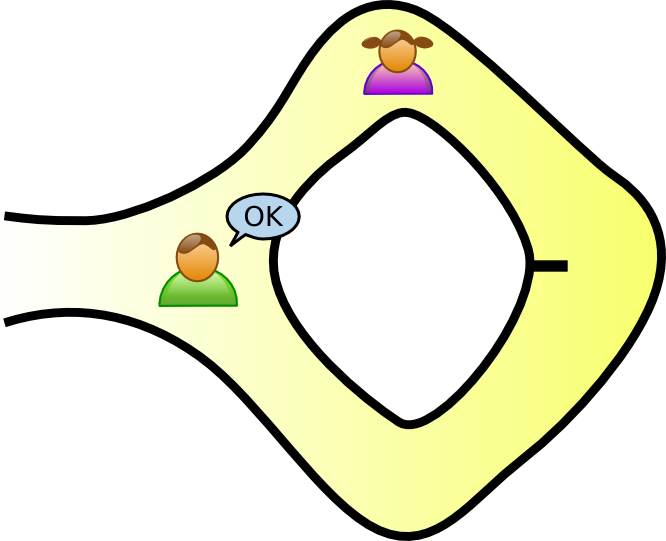
\includegraphics[width=4cm]{./chapters/1.state-of-art/images/5.3.alibaba_cave.png}
        \label{fig:alibaba-cave3}
        \captionsetup{justification=centering}
    \end{subfigure}
    \caption{ZKP: Interazione tra Peggy e Victor}
    \label{fig:alibaba-cave2_3}
\end{figure}
Victor accetta la proposta, ma con una condizione: il processo dovrà essere
ripetuto più volte. Dopo diversi tentativi, Victor si convince che Peggy conosca effettivamente il segreto per superare
la barriera. Possiamo calcolare il grado di fiducia di Victor utilizzando la distribuzione binomiale, dove la probabilità di
successo p è del 50\% e il numero totale di prove n è 10. La probabilità di indovinare correttamente tutte le 10 scelte
di Victor è data dalla seguente formula: \(P = p^n = 0,5^{10} = 0,0009765625\)

L'esempio proposto è molto efficace nel far comprendere come sia possibile dimostrare il possesso o la conoscenza di un
informazione senza rivelarla. Nell’articolo citato inoltre si prevendono diversi scenari in cui una o entrambe le parti
potrebbero essere disoneste. Per gestire tali situazioni, è possibile applicare una procedura denominata "trusted
setup", che verrà approfondita nelle sezioni relativa alle prove non interattive \hyperref[sec:non-interactive]{[Non-Interactive]}.

\subsection{Succinct}
Una dimostrazione di tipo succinct che potremmo tradurre con la parola concisa, è una prova in cui sia la dimensione
della prova che il tempo necessario per verificarla crescono molto più lentamente rispetto alla computazione da
verificare. Ad esempio se Peggy volesse provare a Victor di possedere un array composto da un milione di elementi, dove
ogni elemento è uguale all’indice dell’array più uno.

\begin{equation}
a = [1,2,3,...,1000000]
\end{equation}

Una prova di tipo succinct, così come definita, non può essere realizzata attraverso un processo di controllo "uno per
uno" degli elementi dell'array. Questo perché, se così fosse, si otterrebbe un processo che richiederebbe tanto tempo e
spazio di memoria quanto il calcolo effettuato per generare l'array. Una possibile miglioria rispetto al calcolo puntuale
potrebbe essere quella di campionare l'array in un punto casuale e controllare se l'elemento selezionato rispetta la
regola. \\
Dopo un singolo campionamento, il grado di fiducia di Victor rispetto ad Peggy sarebbe di soli 0,0001\%, ovvero un
milionesimo. Se in uno qualsiasi dei campionamenti effettuati Victor dovesse prelevare un numero non congruo, la
dimostrazione verrebbe invalidata completamente, senza bisogno di ulteriori controlli. È possibile aumentare il grado di
fiducia del verificatore eseguendo più controlli, ma anche in questo caso, le prove generate da dimostratori disonesti
in cui uno o pochi elementi sono errati all'interno dell'intera prova, richiederebbero un numero eccessivo di passaggi
per raggiungere un grado di fiducia accettabile, rendendo cosi questo secondo approccio fragile e non attuabile.

\begin{figure}[H]
    \centering
    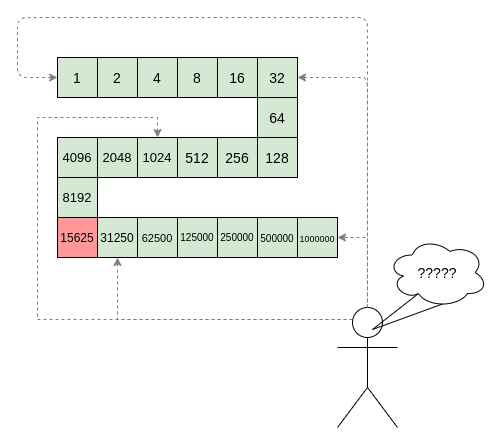
\includegraphics[width=9cm]{./chapters/1.state-of-art/images/6.hope_evaluation.png}
    \label{fig:hope-evaluation}
    \captionsetup{justification=centering}
    \caption{zk-SNARK: verifica a tentativi}
\end{figure}

\subsubsection{Polinomi}

Per trovare una soluzione al problema, è necessario fare riferimento ai polinomi, in particolare alla tecnica
crittografica nota come "polynomial commitments". Questa tecnica ci consente di generare delle funzioni hash per i
polinomi, chiamate "polynomial commitment", sulle quali è ancora possibile effettuare operazioni algebriche. Ciò
significa che possiamo eseguire operazioni sui polinomi senza conoscerli, attraverso i commitment. L'utilizzo di questa
tecnica ci fornisce notevoli vantaggi durante la fase di verifica, infatti la possibilità di verificare le informazioni
del dimostratore senza dover operare un controllo puntuale è possibile grazie a una proprietà dei polinomi descritta dal
lemma di Schwartz-Zippel; un risultato importante in teoria della complessità
computazionale e della teoria degli algoritmi, che stabilisce una condizione sufficiente per determinare se un polinomio
multivariato non nullo ha radici in un campo finito.

Per comprendere come questo strumento possa esserci utile, partiamo da un equivalenza intuitiva: ipotizzando di essere
in possesso di due polinomi $f(x_1,...,x_n)$ e $g(x_1,...,x_n)$, chiedersi se $f \equiv g$ è
equivalente a chiedersi se 

\begin{equation}
p(x_1,...x_n) = f(x_1,...x_n)-g(x_1,...x_n) \equiv 0
\end{equation}

L'intuizione su cui possiamo basarci per capire l’utilità del lemma per i nostri fini, è che Victor (il verificatore) abbia il polynomial
commitment  $g(x_1,...,x_n)$ del polinomio corretto $f(x_1,...,x_n)$ e voglia verificare che Peggy (il dimostratore) lo
conosca. \clearpage
Sotto queste ipotesi possiamo immaginare un semplice protocollo di esempio dove:
\begin{enumerate}
    \item  Victor sceglie un punto qualsiasi $s$ e valuta il suo polynomial commitment in $s$, e ottiene $g(s_1,...,s_n)$.
    \item  Victor invia $s$ a Peggy che provvederà a valutare il suo polinomio in $s$, e ottiene $f(s_1,...,s_n)$.
    \item  Peggy invia il risultato della sua valutazione a Victor che la confronta con il suo valore, se i
    valori sono uguali Victor si convince che nel punto $s$ Peggy consce il corretto polinomio.
\end{enumerate}

In questa fase ci potremmo chiedere quale beneficio abbiamo ottenuto passando dalla formulazione dell'array in cui
venivano fatti campionamenti casuali, alla formulazione dei polinomi in cui vengono fatte valutazioni del polinomio in
variabili casuali. Il beneficio è dovuto al lemma di Schwartz-Zippel, che permette di dimostrare che:

Prendendo un polinomio $p(x_1,...,x_n$) di grado $d > 1$ con coefficienti in un campo finto $\mathbb{K}$, prendendo 
$S \subset \mathbb{K}$ e $r_1,...,r_n \in S$ scelti in modo arbitrario, allora se $p(x_1,...,x_n$) non è il polinomio nullo
abbiamo che $p(r_1,...,r_n) = 0$ con probabilità $\le \ d/|S|$

Nell'immagine sottostante si può osservare che prendendo un polinomio qualunque nel campo finito $\mathbb{K}$, la
probabilità che il polinomio valutato in un punto casuale sia uguale a 0 differisce di poco se calcolata con la
definizione classica di probabilità o con il lemma di Schwartz-Zippel, tuttavia il calcolo attraverso la seconda formula è molto più immediato.
\begin{figure}[H]
    \centering
    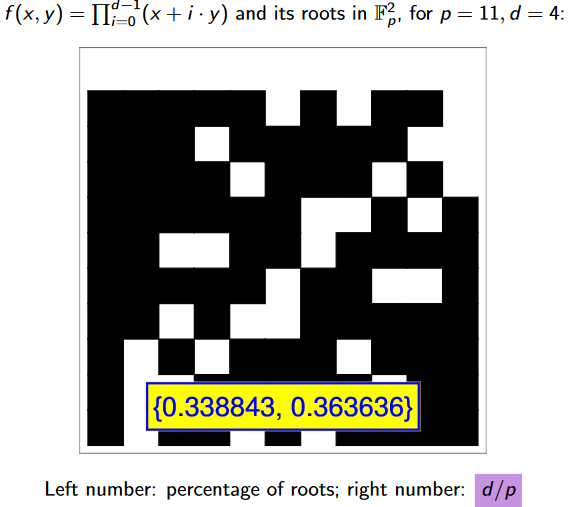
\includegraphics[width=10cm]{./chapters/1.state-of-art/images/7.schwartz_zippel_lemma.png}
    \label{fig:schwartz-zippel-lemma}
    \captionsetup{justification=centering}
    \caption{Visuallizzazione del lemma di Schwartz-Zippel, tratta da \cite{23-schwartz-zippel}}
\end{figure}
\clearpage

La conseguenza del lemma, è che la probabilità di trovare una radice del polinomio in un gruppo di valori appartenenti al
campo è inferiore o uguale al rapporto tra il grado del polinomio e la cardinalità del gruppo di elementi selezionati.
Operazione di rapporto che risulta molto più veloce da calcolare di un controllo puntuale. Inoltre, se decidessimo di ripetere il processo di
selezione degli $r_1,...,r_n \in S$ un numero k di volte otterremo che la probabilità che $p(r^k_1,...,r^k_n) = 0$
sarebbe obbligatoriamente $\le \ (d/|S|)^k$  e per valori di $S$ abbastanza grandi il il rapporto tende molto velocemente
a 0. Intuitivamente il lemma ci dimostra che se un'equazione che coinvolge alcuni polinomi è vera in una coordinata
selezionata arbitrariamente, allora è quasi certamente vera per i polinomio nel suo insieme.

\subsubsection{Come calcolare i polinomi}

Una volta compreso il vantaggio nell'affrontare il problema mediante l'utilizzo dei polinomi, possiamo
procedere alla descrizione del processo che ci permette di ottenere tali polinomi.

\begin{figure}[H]
    \centering
    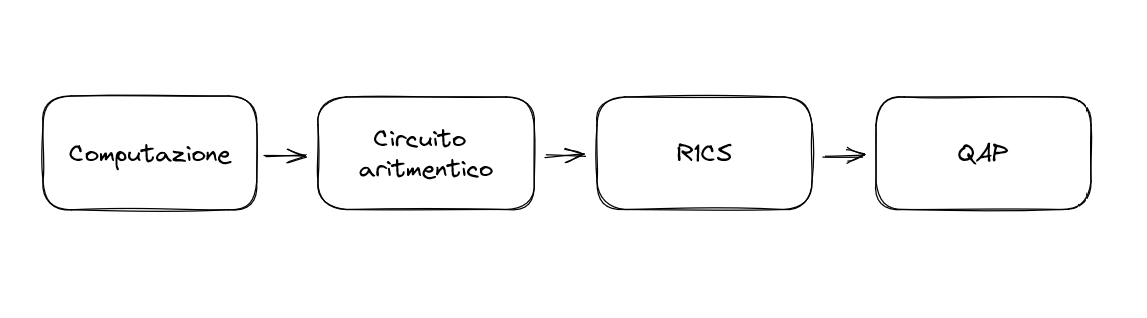
\includegraphics[width=14cm]{./chapters/1.state-of-art/images/8.comp_qap.png}
    \label{fig:comp-qap}
    \captionsetup{justification=centering}
    \caption{Step Circuito - QAP}
\end{figure}

Per illustrare in dettaglio i passaggi che conducono dalla computazione alla rappresentazione polinomiale desiderata,
ovvero la QAP (Quadratic Arithmetic Programs), utilizzeremo un compilatore scritto in Rust\footnote{\url{https://www.rust-lang.org}} chiamato Circom\footnote{\url{https://docs.circom.io/}}

\begin{enumerate}
    \item  La prima fase, ovvero il passaggio dalla computazione al circuito algebrico, può essere un processo non immediato,
    soprattutto quando si trattano computazioni articolate. A titolo di esempio, consideriamo la computazione $2*x^2=18$ con
    l'ovvia soluzione da dimostrare $x=3$. Per ottenere un circuito algebrico a partire da questa computazione, si può
    procedere come segue:\clearpage
        
    \begin{figure}[H]
        \centering
        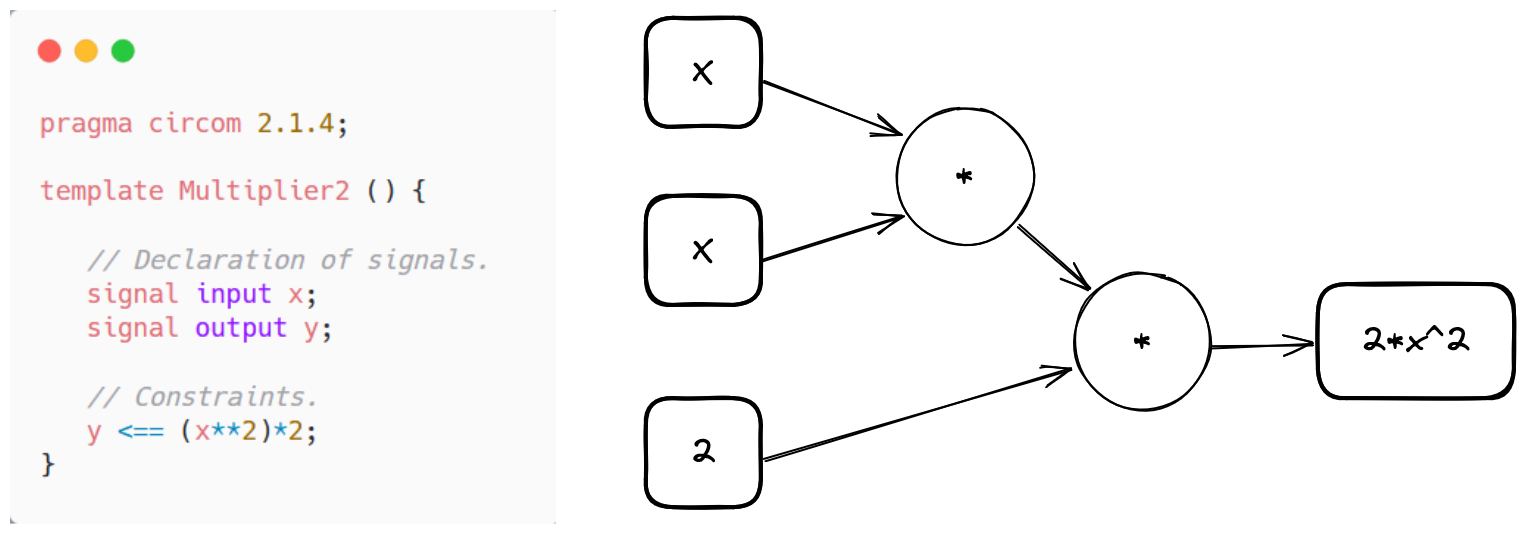
\includegraphics[width=14cm]{./chapters/1.state-of-art/images/9.comp_circ.png}
        \label{fig:comp-circ}
        \captionsetup{justification=centering}
        \caption{Codice esemplificativo per la creazione di un circuito algebrico}
    \end{figure}

    \item  Ora per proseguire dobbiamo trasformare il nostro circuito algebrico in un formato chiamato R1CS. R1CS è un
    formato in cui ogni vincolo (gate del circuito) viene espresso tramite in una terna di vettori (a,b,c) e sul quale viene
    calcolato un vettore chiamo $s$ che rappresenta la soluzione del sistema di vincoli R1CS. Il vettore $s$ è
    costruito nel seguente modo:
    $$
    s \cdot a * s \cdot  b - s \cdot  c = 0
    $$
    
    dove con il simbolo $\cdot$  si rappresenta il prodotto scalare. Continuando con il nostro esempio dal circuito
    precedente possiamo calcolare le terne di vettori $(a,b,c)$ per i due gate
    \begin{gather*}
        A =
        \begin{bmatrix}
        0 & 1 & 0 & 0 \\
        0 & 0 & 0 & 1 \
        \end{bmatrix}
        \qquad
        B =
        \begin{bmatrix}
        0 & 1 & 0 & 0 \\
        2 & 0 & 0 & 0 \
        \end{bmatrix}
        \qquad
        C =
        \begin{bmatrix}
        0 & 0 & 0 & 1 \\
        0 & 0 & 1 & 0 \
        \end{bmatrix}
    \end{gather*}
        
    Possiamo osservare che per ognuno dei due gate del circuito, sono stati creati una terna di vettori $(a,b,c)$ di
    dimensione 4, la dimensione dei vettori è dovuta al numero di variabili del circuito. \\
    Per quanto riguarda il vettore $s$, esso viene calcolato a partire dal vettore delle variabili,
    inserendo al posto di ogni variabile il valore assunto durante la valutazione del circuito. In questo modo, il
    vettore $s$ rappresenta la soluzione del sistema R1CS.

    \begin{gather*}
        \text{Vettore variabili} =
        \begin{bmatrix}
            one, & x, & out, & sym_1 \\
        \end{bmatrix}
        \\
        \\
        \text{Vettore} \ s =
        \begin{bmatrix}
        1 & 3 & 18 & 9 \\
        \end{bmatrix}
    \end{gather*}

    Possiamo vedere che $sym_1$ è una variabile creata per spezzare il calcolo di $2*x^2$ in due diversi vincoli più
    semplici questa procedura viene chiamata "Flattening" (appiattimento), mentre $one$ è una variabile di sistema
    utilizzata per effettuare operazioni algebriche come la moltiplicazione o la somma per gli elementi del campo. Per
    verificare che il vettore $s$ sia effettivamente una soluzione del sistema di vincoli R1CS, è possibile calcolare la
    formula precedente per ogni gate del circuito.

    \begin{figure}[H]
        \centering
        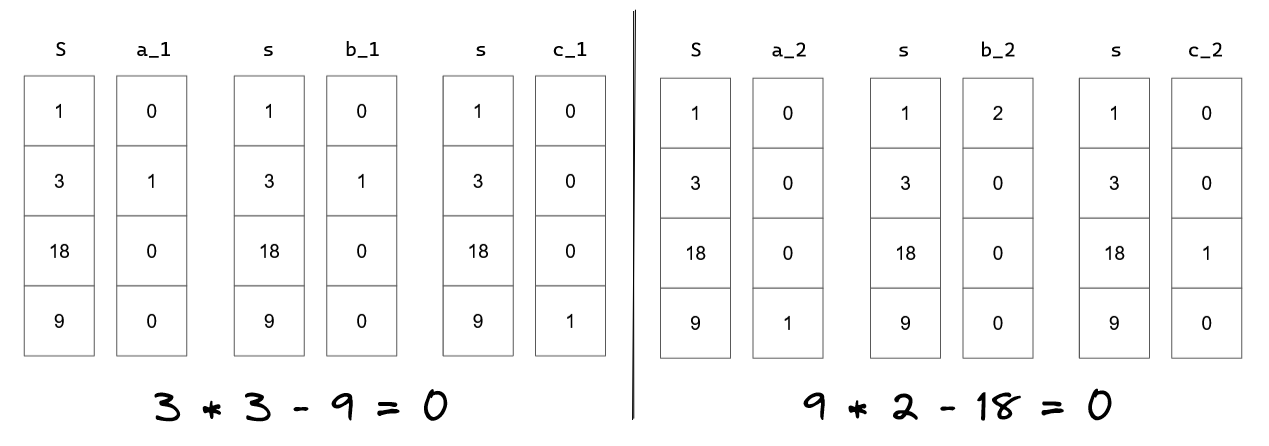
\includegraphics[width=15cm]{./chapters/1.state-of-art/images/10.check_r1cs.png}
        \label{fig:check-r1cs}
        \captionsetup{justification=centering}
        \caption{Controllo dei vincoli R1CS}
    \end{figure}

    Visto che il risultato dell'operazione è 0 possiamo dire che $s$ è una soluzione del sistema R1CS, e quindi che il
    nostro valore $x=3$ che compone il vettore soluzione è corretto. Al pari del calcolo puntuale degli esempi
    precedenti, questa operazione di verifica per circuiti con molti gate non può essere percorribile.

    \item  Il processo di trasformazione dal formato R1CS al formato QAP è il più complesso e richiede l'utilizzo di una
    tecnica chiamata interpolazione di Lagrange. L'idea principale è quella di costruire dei polinomi tali che se
    valutati nelle coordinate relative ai vincoli, restituiscano i valori dei vettori corrispondenti. Il processo per
    ottenere i polinomi si basa su una procedura iterativa su i vettori delle matrici $A,B$ e $C$. 
    Applicando il processo al nostro esempio otteniamo le seguenti matrici di polinomi:
    \begin{gather*}
        \text{Ap} =
        \begin{bmatrix}
        0x^2+0x \\
        -1x^2+2x \\
        0x^2+0x \\
        1x^2-1x \
        \end{bmatrix}
        \qquad
        \text{Bp} =
        \begin{bmatrix}
        2x^2-2x \\
        -1x^2+2x \\
        0x^2+0x \\
        0x^2+0x \
        \end{bmatrix}
        \qquad
        \text{Cp} =
        \begin{bmatrix}
        0x^2+0x \\
        0x^2+0x \\
        1x^2-1x \\
        -1x^2+2x \
        \end{bmatrix}
    \end{gather*}    
    Questi polinomi sono costruiti in modo tale che valutandoli in x = 1 (coordinata del primo vincolo) otteniamo i valori corrispondenti ai vettori del
    primo vincolo
    \begin{gather*}
        \text{Ap} =
        \begin{bmatrix}
        0&\
        1&\
        0&\
        0\
        \end{bmatrix}
        \qquad
        \text{Bp} =
        \begin{bmatrix}
        0&\
        1&\
        0&\
        0\
        \end{bmatrix}
        \qquad
        \text{Cp} =
        \begin{bmatrix}
        0&\
        0&\
        0&\
        1\
        \end{bmatrix}
    \end{gather*}
    grazie a questa formato ora se volessimo verificando i vincoli tramite la formula precedente avremmo
    
    $$
    A(x)*B(x)-C(x)=P(x)
    $$
    
    dove $P(x)$ non è obbligatoriamente il polinomio nullo. Tuttavia se la dimostrazione è corretta $P(x)$ deve avere delle
    radici in tutte le coordinate corrispondenti ai vincoli. Per verificarlo non abbiamo bisogno di controllare tutti i
    punti, perché lavorando con i polinomi possiamo sfruttare il lemma di Schwartz-Zippel per valutare la condizione
    molto più velocemente.
\end{enumerate}
    
\subsubsection{Valutazioni sul protocollo}
Fino ad ora abbiamo descritto un processo che ci consente di trasformare i nostri vincoli numerici in polinomi,
permettendoci di calcolare con grande velocità e un elevato grado di certezza la validità dei vincoli imposti. Tuttavia,
il protocollo spiegato in precedenza presenta due falle:

\begin{enumerate}
    \item \textbf{Arbitrarietà}: Nel secondo passaggio del protocollo, Victor condivide con Peggy un punto $s$, che è stato scelto
    casualmente per valutare il polinomio. Tuttavia, passando $s$ in chiaro a Peggy ci si espone al rischio che Peggy
    costruisca un polinomio ad hoc, che soddisfi i vincoli solo nel punto specifico scelto, permettendole così di convincere
    Victor pur non conoscendo il polinomio. Ciò violerebbe il principio di correttezza dei protocolli Zero Knowledge proof.
    \item \textbf{Verificabilità}: la capacità di Peggy di valutare correttamente il polinomio in $s$ non garantisce che essa abbia
    utilizzato effettivamente il polinomio $p$ per restituire il risultato a Victor, In altre parole, non è garantito che Peggy
    abbia utilizzato il polinomio descritto dal polynomial commitment per raggiungere il risultato atteso.
\end{enumerate}

Per affrontare questi due problemi, vengono utilizzate altre tecniche matematiche, denominate Homomorphic Encryption (HH) per
risolvere il primo problema e Knowledge of Coefficient (KC) per risolvere il secondo. In questa sede, si accennerà
brevemente a come è possibile ottenere un Homomorphic Encryption in grado di soddisfare la proprietà di correttezza,
mentre la trattazione del KC non verrà approfondita. È possibile trovare una introduzione ad entrambe le tecniche
in questa serie di articoli \cite{explaining_sanrks}

\subsubsection{Homomorphic Encryption}

L'idea alla base dell'Homomorphic Encryption è quella di costruire un'operazione simile all'operazione di hashing con la
proprietà di poter applicare delle operazioni aritmetiche ai valori criptati senza decifrarli, ovvero ottenere una
funzione $E(x)$ che soddisfi tali proprietà :
\begin{enumerate}
    \item \textbf{Difficoltà di inversione}: Dato un  $E(x)$ sia complesso risalire a $x$
    \item \textbf{Resistenza alle collisioni}: Se $x \ne y \Rightarrow E(x) \ne E(y)$
    \item \textbf{Preservare operazioni aritmetiche}: Se si conoscono E(x) ed E(y), si può generare
    delle espressioni aritmetiche in x e y. Per esempio, si può calcolare E(x+y) da E(x) ed E(y)
\end{enumerate}
\clearpage

\subsection{Non-Interactive}
\label{sec:non-interactive}

Tutti i protocolli Zero Knowledge proof esaminati fino ad ora erano di tipo interattivo. Questo significa che per
generare e verificare la prova, le due parti coinvolte, ovvero il verificatore e il dimostratore, devono interagire in
modo bidirezionale. Ad esempio, nel caso della "grotta", Victor, il verificatore, indicava il passaggio da
intraprendere e Peggy, il dimostratore “rispondeva” uscendo dalla giusta direzione. Mentre nel caso dei
polinomi, il verificatore forniva le coordinate del punto in cui valutare il polinomio e il dimostratore rispondeva con
la valutazione corretta. In alcune situazioni, tuttavia può risultare vantaggioso utilizzare le cosiddette NIZKP, ovvero
le Non-Interactive Zero Knowledge proof, in cui il dimostratore trasmette al verificatore una prova contenente tutte le
informazioni necessarie per la verifica, senza richiedere ulteriori interazioni tra le parti. 

Questa metodologia presenta numerosi vantaggi sia in termini di prestazioni, poiché consente di costruire le prove più
velocemente senza dover attendere la risposta e il tempo di comunicazione, sia in termini di sicurezza, in quanto
l'assenza di uno scambio di messaggi elimina il rischio di intercettazioni da parte di individui malintenzionati.
Inoltre, l'utilizzo di prove NIZKP potrebbe risultare obbligato in quei contesti applicativi in cui la comunicazione in
tempo reale non è possibile. L'adozione di questo tipo di prove comporta però un aumento della complessità, poiché,
essendo privi di interazione, tutto il lavoro di generazione e preparazione alla verifica viene svolto dal dimostratore.
Affinché il dimostratore non sia arbitrariamente libero di agire, generando prove scorrette, è necessario vincolarlo
al rispetto delle regole. 

A tal fine, si utilizza una tecnica nota come "trusted set-up" che consente di generare una Common Reference String
(CRS), ovvero un dato pubblico conosciuto sia dal dimostratore che dal verificatore usato per aggiungere casualità
all’interno della generazione della prova. Sempre riferendoci ai due esempi precedenti, la CRS ottenuta tramite un
trusted set-up consentirebbe di rendere le scelte di Victor nella caverna il più casuali possibile, impedendo ad Peggy
di individuare dei pattern o a entrambi di collaborare per ingannare un terzo osservatore e nel caso dei polinomi,
invece, consentirebbe di rendere aleatoria la scelta del punto in cui valutare il polinomio. 

La procedura di costruzione della CRS rappresenta un passaggio critico per la robustezza del protocollo e dipende
fortemente dal tipo di cerimonia di trusted set-up scelta.

\subsubsection{Modello di affidabilità}

Una cerimonia di trusted set-up è una procedura che viene eseguita una sola volta per generare una CRS che poi potrà
essere utilizzata ogni volta che viene eseguito il protocollo. Il termine "trusted" deriva dal fatto che una o più
persone devono partecipare alla cerimonia in modo “fidato” contribuendo alla creazione della CRS con dei segreti anche
chiamati “toxic waste” che non appena inseriti nella procedura dovranno essere eliminati. \clearpage

Una volta completata l'elaborazione e dopo aver eliminato i segreti, il risultato dell'elaborazione (la CRS) diventa
irreversibile e non può essere riprodotta volontariamente, il che garantisce la sicurezza del protocollo.
\begin{figure}[H]
    \centering
    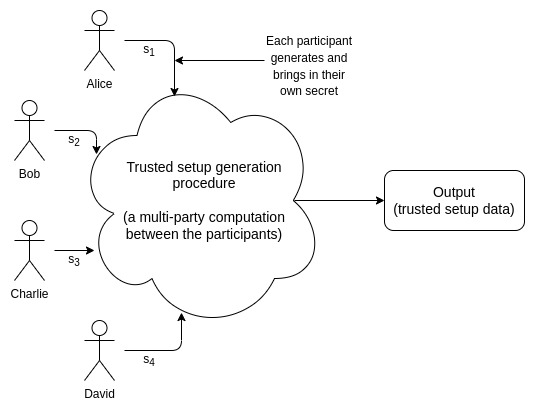
\includegraphics[width=10cm]{./chapters/1.state-of-art/images/11.trusted_setups.png}
    \label{fig:trusted_setups}
    \captionsetup{justification=centering}
    \caption{Immagine generica di una cerimonia di trusted set-up, tratta da \cite{how-do-trusted-setups-work}}
\end{figure}

Se le parti coinvolte non si comportano in modo leale e conservano o pubblicano i loro segreti, la validità della
cerimonia dipenderà dal modello di affidabilità utilizzato dall'algoritmo di trusted set-up. Infatti poiché i protocolli
operano in diversi domini applicativi, non tutti utilizzano lo stesso modello di affidabilità. 

Una trattazione completa dei vari modelli di affidabilità esula dai miei scopi, tuttavia, riducendo la classificazione a due sole proprietà
degli algoritmi, è possibile descrivere brevemente alcune tipologie utili per la trattazione successiva. 

Le due proprietà su cui si basa la classificazione sono il numero di parti fidate che partecipano alla cerimonia (primo numero) e il numero di
parti che devono comportarsi “lealmente” per garantire la segretezza della CRS (secondo numero).

In base a queste proprietà, si possono individuare tre gruppi di interesse (non sono gli unici):
\begin{itemize}
    \item \textbf{1 - 1}: Questo modello è simile a quello utilizzato nei servizi centralizzati, in cui ci si affida a un singolo
    individuo fidato per la gestione dei dati. 
    \item \textbf{N/2 - 1}: La maggior parte delle blockchain utilizza questo modello, in
    cui il processo viene considerato valido se la maggioranza dei partecipanti rimane onesta.
    \item \textbf{1 - N}: In questo modello, è sufficiente che almeno una delle parti rimanga onesta durante la
    cerimonia per garantire la segretezza della CRS.
\end{itemize}

\begin{figure}[H]
    \centering
    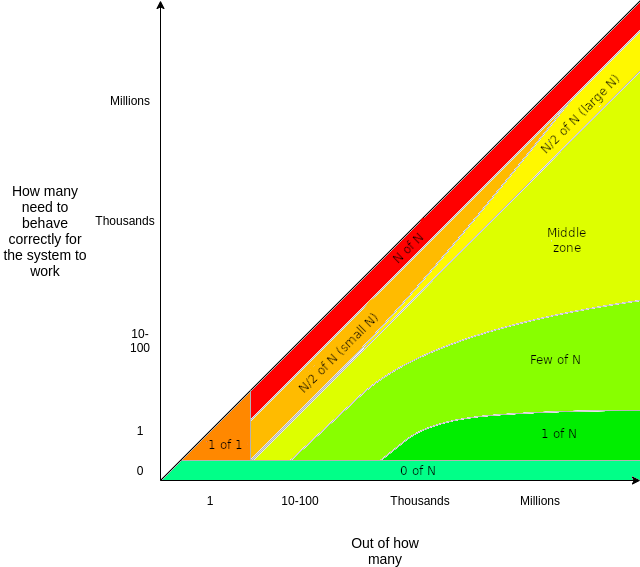
\includegraphics[width=10cm]{./chapters/1.state-of-art/images/12.trusted_models.png}
    \label{fig:trusted_models}
    \captionsetup{justification=centering}
    \caption{Immagine modelli di affidabilità, tratta da \cite{trusted-models}}
\end{figure}

\subsubsection{MPC (multi-party computation)}
La tecnologia MPC (multi-party computation), anche se non è stata ancora esplicitamente menzionata, è alla base dei
trusted set-up. Infatti per generare una CRS sicura e non riproducibile, è necessario coinvolgere molte parti e
garantire che nessuno possa ricavare informazioni sui segreti dei partecipanti o sulla CRS stessa. Per questo motivo la
procedura non si limita a una semplice combinazione dei segreti, ma può essere vista come una "black box" che applica
elaborazioni ai segreti in input e restituisce la CRS in output.

Ogni algoritmo di MPC deve soddisfare due proprietà fondamentali:

\begin{enumerate}
    \item Nel caso in cui uno o più partecipanti disonesti decidano di rivelare il loro segreto, il protocollo MPC deve
    impedire loro di obbligare i partecipanti onesti a rivelare le loro informazioni riservate o influenzare il risultato
    finale.
    \item Nessuno dei partecipanti deve essere in grado di dedurre i segreti degli altri partecipanti dagli elaborati
    del protocollo. In altre parole, il calcolo effettuato dall'algoritmo non deve fornire alcun indizio sui segreti che
    hanno portato al risultato.
\end{enumerate}

\subsubsection{Groth16}
Groth16 è un protocollo Zero Knowledge proof proposto da Jens Groth nell’articolo “On the Size of Pairing-based
Non-interactive Arguments” \cite{10.1007/978-3-662-49896-5_11} pubblicato nel 2016, questo protocollo è diventato molto
diffuso grazie alla sua grande efficienza dal punto di vista computazionale, che permette di creare zk-SNARK
estremamente performanti sia in termini di tempo che di memoria. Tale tecnologia è alla base di progetti come Z-cash\footnote{\url{https://z.cash/}}.

Il trusted set-up su cui si basa Groth16 richiede due fasi distinte:
\begin{enumerate}
    \item Nella prima fase si applica una procedura di trusted set-up chiamata “power of tau” che consiste in una algoritmo MPC
    basato sul modello di affidabilità 1-N che utilizzando le curve ellitiche permette di generare una CRS. Il processo viene
    chiamato powers of tau o Pot perché durante le sue fasi vengono usate le potenze di un numero tao generalmente il 2
    assime ai contributi dei partecipanti, per generare punti casuali e ottener una CRS. il numero N di partecipati per una
    cerimonia di tipo power of tau può essere dell'ordine del migliaio rendendo cosi la cerimonia molto
    sicura, in quanto basta che almeno uno di essi mantenga il segreto per far si che la CRS rimanga valida. Questo
    procedimento deve essere svolto una volta sola e deve essere combinato con il processo della fase successiva.
    \begin{figure}[H]
        \centering
        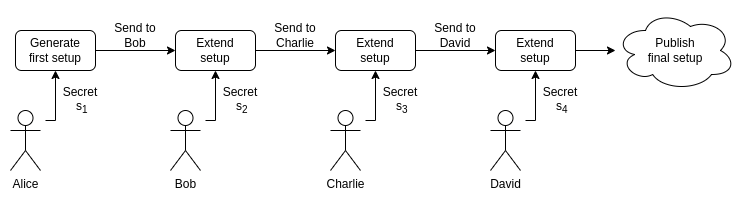
\includegraphics[width=13cm]{./chapters/1.state-of-art/images/13.power_of_tao.png}
        \label{fig:powers_of_tao}
        \captionsetup{justification=centering}
        \caption{Immagine cerimonia power of tau, tratta da \cite{how-do-trusted-setups-work}}
    \end{figure}
    \item Nella seconda fase invece viene elaborato un trusted set-up dipendente dalla computazione che si vuole provare (o
    meglio dipendete dal circuito). Quindi questa fase deve essere riprodotta dal dimostratore ogni volta che la
    dimostrazione cambia. Non entrerò nei dettagli implementativi, ma in questa fase viene utilizzata l' euristica di Fiat-Shamir
    , che permette di scegliere il punto in cui valutare il polinomio, che descrive la computazione, senza che il
    dimostratore possa interferire. Il punto viene scelto sulla base dei calcoli fatti per ottenere il polinomio stesso. È
    intuitivo comprendere che se il dimostratore volesse falsificare la prova, non potrebbe farlo, perché per scegliere
    arbitrariamente un polinomio che soddisfa un determinato vincolo in $s$, dovrebbe conoscerene a priori il valore, ma essendo
    $s$ derivato dal polinomio stesso questo non è possibile.
\end{enumerate}

Indubbiamente il fatto che la robustezza della tecnologia zk-SNARK sia subordinata a una procedura cosi elaborata è uno
svantaggio, infatti esistono, protocolli di Zero Knowledge proof che non necessitano di una fase di trust set-up
iniziale. Bulletproof e le STARK (Scalable Transparent Arguments of Knowledge), ad esempio, non richiedono alcuna
configurazione di questo tipo, ciò nonostante, le tecnologie  zk-SNARK basate su Groth16 risultano essere più performati in termini di
tempi di verifica il che le rende molto più diffuse delle altre tecnologie.
\begin{figure}[H]
    \centering
    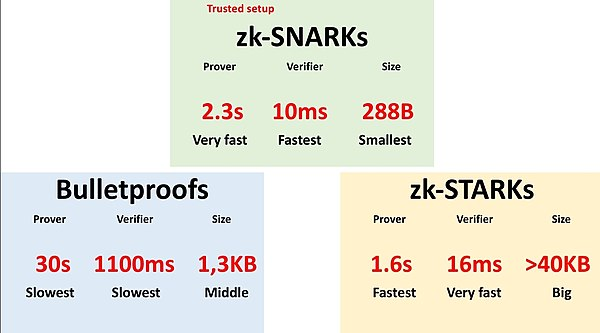
\includegraphics[width=13cm]{./chapters/1.state-of-art/images/14.diff_zk.png}
    \label{fig:different_zk}
    \captionsetup{justification=centering}
    \caption{Immagine prestazioni NIZKP a confronto, tratta da \cite{non_interactive_zero_knowledge_proof}}
\end{figure}